\documentclass[11pt,a4paper]{article}
\usepackage[utf8]{inputenc}
\usepackage[T1]{fontenc}
\usepackage{amsmath,amssymb}
\usepackage{booktabs}
\usepackage{graphicx}
\graphicspath{{figures/}}
\usepackage{hyperref}
\usepackage{natbib}
\usepackage{xcolor}
\usepackage{multirow}
\usepackage{geometry}
\geometry{margin=1in}

\title{Language Models Don't Know What Time It Is}

\author{
  Neil Tripathi \\
  Independent Research
}

\date{March 2026}

\begin{document}
\maketitle

% ============================================================
\begin{abstract}
Across controlled stale-context decision tasks, language models show near-zero sensitivity (0--8\%) to elapsed time unless age is explicitly represented in the prompt.
We evaluate seven models -- from Mistral-7B to GPT-5.4 and Claude Opus 4.6 -- on counterfactual scenario pairs tested with and without elapsed-time annotations.
Without annotations, models produce the same action regardless of whether context is 30 seconds old or 4 hours old.
Adding a single natural-language annotation (``Time since observed: 4 hours ago'') raises switch sensitivity to 31--100\% and substantially reduces false trust in stale information.

We call this the \emph{temporal blind spot}: the consistent inability of language models, across the models and tasks we tested, to assess context reliability based on age -- despite possessing latent temporal reasoning that activates when elapsed time is made salient.
On a 96-case generated benchmark, GPT-5.4 reaches 66\% switch sensitivity with explicit annotations, Claude Opus 4.6 reaches 64\%, and Claude Sonnet reaches 63\%, with false trust dropping from 27--42\% to 7--14\%.
The fix requires no retraining -- only a prompt-layer change.
\end{abstract}

% ============================================================
\section{Introduction}
\label{sec:intro}

LLM-based agents routinely operate over context that was retrieved, cached, or observed at some earlier point in time.
A flight status checked 30 seconds ago is reliable; the same status checked 4 hours ago is not.
Yet language models receive this context as flat text with no indication of age.
The model has no way to know whether it is looking at information from moments ago or from last week.

This paper demonstrates that this is not merely an inconvenience -- it is a consistent failure mode across every model and task we tested.
We evaluate seven frontier and mid-tier models across two benchmarks: 18 hand-crafted scenarios tested across four prompting conditions, and a larger 96-case generated benchmark focused on the two most capable models (1{,}406 API calls in total).
Without elapsed-time annotations, all models exhibit near-zero switch sensitivity (0--8\%): given the same fact observed 30 seconds ago versus 4 hours ago, they almost always give the same answer.

The fix is simple.
Adding a single line -- ``Time since this information was observed: 4 hours ago'' -- causes models to differentiate fresh from stale context.
On a 96-case generated benchmark, GPT-5.4 and Claude Opus 4.6 reach 64--66\% switch sensitivity, with false trust dropping from 27--42\% to 7--14\%.

We call this the \emph{temporal blind spot}: the inability of language models to assess context reliability based on age, despite possessing latent temporal reasoning capabilities that activate when elapsed time is made explicit.

\paragraph{Contributions.}
\begin{enumerate}
    \item We design a \textbf{counterfactual evaluation framework} that isolates the effect of elapsed-time annotations on stale-context detection, controlling for prompt content.
    \item We show that the temporal blind spot is \textbf{consistent across seven models spanning three providers and four capability tiers}, and does not diminish with scale.
    \item We demonstrate that a \textbf{single natural-language time annotation} substantially reduces the blind spot, requiring no model retraining -- only a prompt-layer change.
    \item We identify a \textbf{staleness-caution tradeoff}: smaller models over-correct by refreshing stable facts, suggesting that time awareness requires calibration against fact volatility.
\end{enumerate}

% ============================================================
\section{Related Work}
\label{sec:related}

\paragraph{Temporal reasoning in LLMs.}
Prior work on temporal reasoning in language models has focused primarily on knowledge-oriented tasks: ordering events on a timeline \citep{ning2018multi}, resolving temporal expressions \citep{zhou2019going}, and answering questions about when events occurred \citep{dhingra2022time}.
More recent benchmarks test whether models can track entity states over time \citep{lazaridou2021mind,luu2022time} and whether their parametric knowledge reflects temporal dynamics \citep{jang2022temporalwiki,kasai2023realtime}.
Our work addresses a different question: not whether models \emph{know} temporal facts, but whether they can \emph{use} elapsed time to decide if cached context is still trustworthy -- a decision-making task rather than a knowledge task.

\paragraph{Time-aware memory and retrieval.}
Several agent architectures maintain timestamped memory stores \citep{park2023generative,zhong2024memorybank}, but the focus is on memory retrieval relevance rather than on whether the model can assess the reliability of information based on its age.
RAG systems \citep{lewis2020retrieval} retrieve context but rarely annotate it with observation time, and time-aware retrieval work \citep{zhang2023retrieve} has focused on recency-biased ranking rather than on the downstream effect of temporal metadata on model decisions.
Our results suggest that retrieval recency is not sufficient -- the model must also be told \emph{how old} the retrieved context is.

\paragraph{Tool use and agent decision-making.}
Tool-using agents \citep{schick2023toolformer,qin2023toolllm} must decide when to invoke tools versus rely on cached observations.
This decision is inherently temporal: a tool output from seconds ago may be trustworthy, while the same output from hours ago may not.
To our knowledge, no prior work has systematically evaluated whether models condition this decision on elapsed time.

\paragraph{Calibration, abstention, and selective prediction.}
Work on selective prediction \citep{kamath2020selective} and calibrated uncertainty \citep{kadavath2022language} studies when models should abstain from answering.
We add a temporal dimension: models should abstain or refresh specifically when context is \emph{old enough to be unreliable}, and the appropriate threshold depends on fact volatility.
This connects to the broader literature on knowing what you don't know \citep{yin2023large}, extended here to knowing when what you knew may no longer hold.

% ============================================================
\section{Evaluation Framework}
\label{sec:framework}

\subsection{Counterfactual Design}

Our evaluation is built on \emph{counterfactual pairing}: each scenario appears in both a \textbf{fresh} version (short elapsed time, correct action: trust the context) and a \textbf{stale} version (long elapsed time, correct action: refresh).
The conversation text, query, and available actions are identical across the pair -- only the elapsed time differs.
This design controls for prompt content and isolates the effect of temporal information on model decisions.

\subsection{Test Scenarios}

We construct 18 hand-crafted scenarios spanning five categories:
\begin{itemize}
    \item \textbf{High volatility} (8 cases): flight status, stock prices, weather, traffic, restaurant availability, crypto prices, delivery tracking, sports scores
    \item \textbf{Low volatility} (4 cases): birthday, home address, capital cities, programming syntax
    \item \textbf{Medium volatility} (3 cases): CEO identity, software versions, medication dosage
    \item \textbf{Deadline-aware} (2 cases): meeting room with imminent meeting, auction bid near closing
    \item \textbf{Memory retrieval} (1 case): conflicting user preferences at different times
\end{itemize}

Each scenario uses realistic, factually accurate content.
Fresh elapsed times range from 20 seconds to 2 hours; stale times range from 3 hours to 2 years, calibrated to each fact type's natural volatility.

\subsection{Prompting Conditions}

Models are tested in four conditions:
\begin{enumerate}
    \item \textbf{No time}: No temporal information. Model sees context + query only.
    \item \textbf{Implicit}: Elapsed time mentioned casually in a context header (``observed 3 hours ago'').
    \item \textbf{Explicit}: Clear, separated annotation: ``Time since this information was observed: 3 hours ago.''
    \item \textbf{Prompted}: Explicit time plus a system prompt instructing the model to consider staleness.
\end{enumerate}

\subsection{Action Space}

Models choose from five actions:
(A)~answer directly from cached context,
(B)~refresh/look up the information again,
(C)~retrieve from memory for more context,
(D)~ask a clarifying question, or
(E)~abstain.
All calls use temperature 0 for reproducibility.

\subsection{Primary Metric: Switch Sensitivity}

\textbf{Switch sensitivity} measures whether the model changes its action across the counterfactual pair when the correct action changes.
For each scenario where fresh and stale have different correct actions (e.g., ``answer directly'' vs.\ ``refresh''), we check whether the model's prediction also differs.

A model with 0\% switch sensitivity always produces the same action regardless of elapsed time.
A model with 100\% always differentiates fresh from stale when it should.

\subsection{Models Tested}

We evaluate seven models spanning three providers and four capability tiers:
\begin{itemize}
    \item \textbf{OpenAI}: GPT-4o, GPT-4o-mini, GPT-5.4
    \item \textbf{Anthropic}: Claude Sonnet 4, Claude Haiku 4.5, Claude Opus 4.6
    \item \textbf{Local}: Mistral-7B-Instruct-v0.2 (16\,GB VRAM)
\end{itemize}

We additionally evaluate GPT-5.4 and Claude Opus 4.6 on a \textbf{96-case generated benchmark} produced programmatically from our taxonomy of 16 fact types, balanced across four volatility levels (24 cases each).
This larger benchmark tests whether the effect observed on hand-crafted scenarios generalises to a broader, more diverse set.

Total evaluation: 1{,}406 API calls across all models, conditions, scenarios, and fresh/stale variants (638 on the 18-case benchmark, 768 on the 96-case benchmark).

% ============================================================
\section{Results}
\label{sec:results}

Table~\ref{tab:frontier} presents the full results across all models and conditions.

\begin{table}[t]
\centering
\caption{Results across seven models. The top section shows five models evaluated on 18 hand-crafted scenarios across up to four prompting conditions. The bottom section shows GPT-5.4 and Claude Opus 4.6 evaluated on a larger 96-case generated benchmark (no-time and explicit conditions only).}
\label{tab:frontier}
\small
\begin{tabular}{llccccc}
\toprule
\textbf{Model} & \textbf{Condition} & \textbf{$n$} & \textbf{Accuracy} & \textbf{Switch Sens} & \textbf{False Trust} & \textbf{Unnec.\ Refresh} \\
\midrule
\multicolumn{7}{l}{\emph{18 hand-crafted scenarios, up to 4 conditions}} \\
\midrule
\multirow{4}{*}{GPT-4o}
  & No time   & 34  & 0.529 & 0.077 & 0.692 & 0.000 \\
  & Implicit  & 36  & 0.611 & 0.308 & 0.308 & 0.238 \\
  & Explicit  & 36  & 0.833 & 1.000 & 0.000 & 0.048 \\
  & Prompted  & 36  & 0.889 & 0.923 & 0.000 & 0.048 \\
\midrule
\multirow{2}{*}{GPT-4o-mini}
  & No time   & 34  & 0.618 & 0.000 & 1.000 & 0.000 \\
  & Explicit  & 36  & 0.778 & 0.538 & 0.462 & 0.000 \\
\midrule
\multirow{4}{*}{Claude Sonnet 4}
  & No time   & 34  & 0.618 & 0.000 & 0.846 & 0.095 \\
  & Implicit  & 36  & 0.528 & 0.154 & 0.077 & 0.476 \\
  & Explicit  & 36  & 0.833 & 0.769 & 0.000 & 0.143 \\
  & Prompted  & 36  & 0.694 & 0.462 & 0.000 & 0.333 \\
\midrule
\multirow{4}{*}{Claude Haiku 4.5}
  & No time   & 34  & 0.588 & 0.000 & 0.538 & 0.238 \\
  & Implicit  & 36  & 0.583 & 0.308 & 0.000 & 0.381 \\
  & Explicit  & 36  & 0.500 & 0.385 & 0.000 & 0.429 \\
  & Prompted  & 36  & 0.528 & 0.154 & 0.000 & 0.524 \\
\midrule
\multirow{4}{*}{Mistral-7B}
  & No time   & 34  & 0.618 & 0.000 & 1.000 & 0.000 \\
  & Implicit  & 36  & 0.639 & 0.154 & 0.846 & 0.000 \\
  & Explicit  & 36  & 0.694 & 0.308 & 0.692 & 0.000 \\
  & Prompted  & 36  & 0.361 & 0.000 & 0.000 & 1.000 \\
\midrule
\multicolumn{7}{l}{\emph{96 generated scenarios, 2 conditions}} \\
\midrule
\multirow{2}{*}{GPT-4o}
  & No time   & 192 & 0.526 & 0.034 & 0.339 & 0.318 \\
  & Explicit  & 192 & 0.661 & 0.407 & 0.136 & 0.252 \\
\midrule
\multirow{2}{*}{GPT-5.4}
  & No time   & 192 & 0.573 & 0.051 & 0.424 & 0.290 \\
  & Explicit  & 192 & 0.760 & 0.661 & 0.102 & 0.131 \\
\midrule
\multirow{2}{*}{Claude Sonnet 4}
  & No time   & 192 & 0.547 & 0.000 & 0.390 & 0.318 \\
  & Explicit  & 192 & 0.682 & 0.627 & 0.068 & 0.178 \\
\midrule
\multirow{2}{*}{Claude Opus 4.6}
  & No time   & 192 & 0.547 & 0.000 & 0.271 & 0.383 \\
  & Explicit  & 192 & 0.745 & 0.644 & 0.085 & 0.150 \\
\bottomrule
\end{tabular}
\end{table}

\begin{figure}[t]
\centering
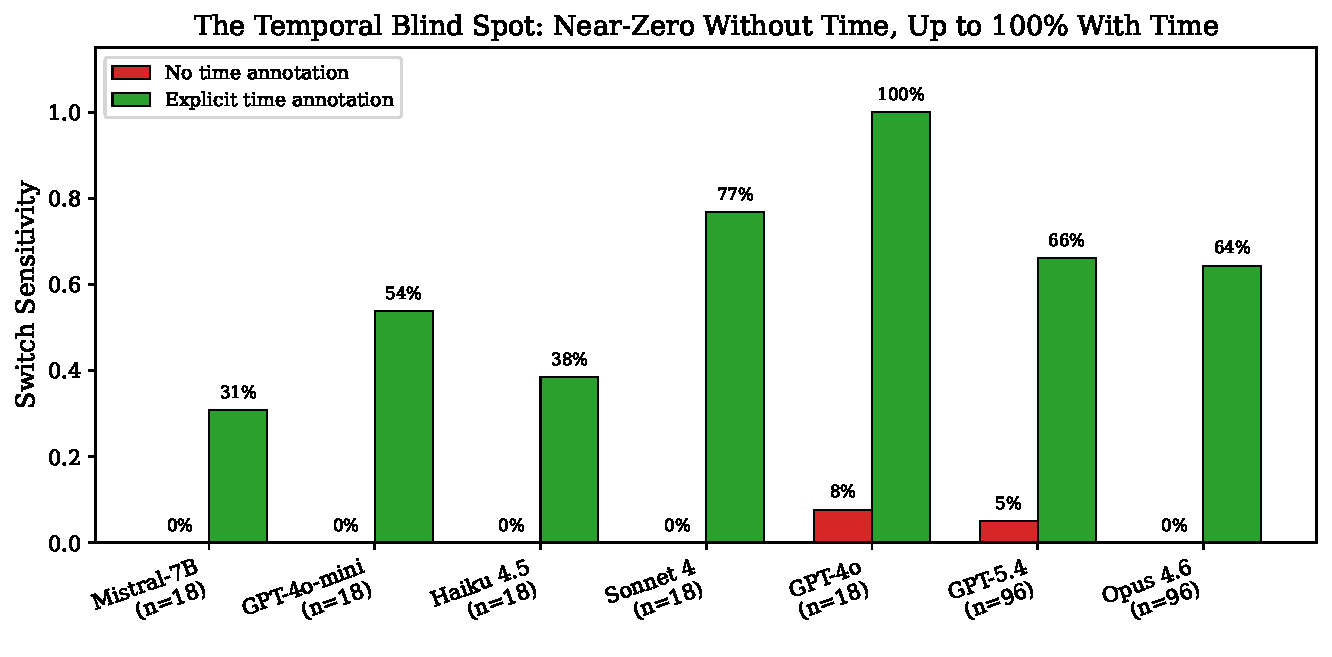
\includegraphics[width=\textwidth]{fig1_blind_spot.pdf}
\caption{Switch sensitivity across all seven models with and without explicit elapsed-time annotations. Without time, all models fall in the 0--8\% range. With explicit time, the most capable models reach 100\%.}
\label{fig:blind_spot}
\end{figure}

\subsection{Finding 1: Low Temporal Sensitivity Without Annotations}

In the no-time condition, all seven models exhibit near-zero switch sensitivity (0--8\%).
They produce effectively the same action regardless of whether context is 30 seconds old or 4 hours old.

The failure is not subtle.
GPT-4o-mini and Mistral-7B achieve 100\% false trust in the no-time condition on the 18-case benchmark -- they always tell the user to trust stale information.
Claude Sonnet shows a false trust rate of 84.6\%.
On the larger 96-case benchmark, GPT-5.4 shows 42.4\% false trust and Claude Opus 4.6 shows 27.1\%.
Even GPT-5.4 -- the most capable model at the time of evaluation -- manages only 5.1\% switch sensitivity without time annotations.

This is consistent with a \emph{representation gap} rather than a capacity limitation.
These models can reason about time when asked ``When did X happen?''
They simply do not use temporal context to assess whether cached information is still reliable, absent an explicit cue.

\begin{figure}[t]
\centering
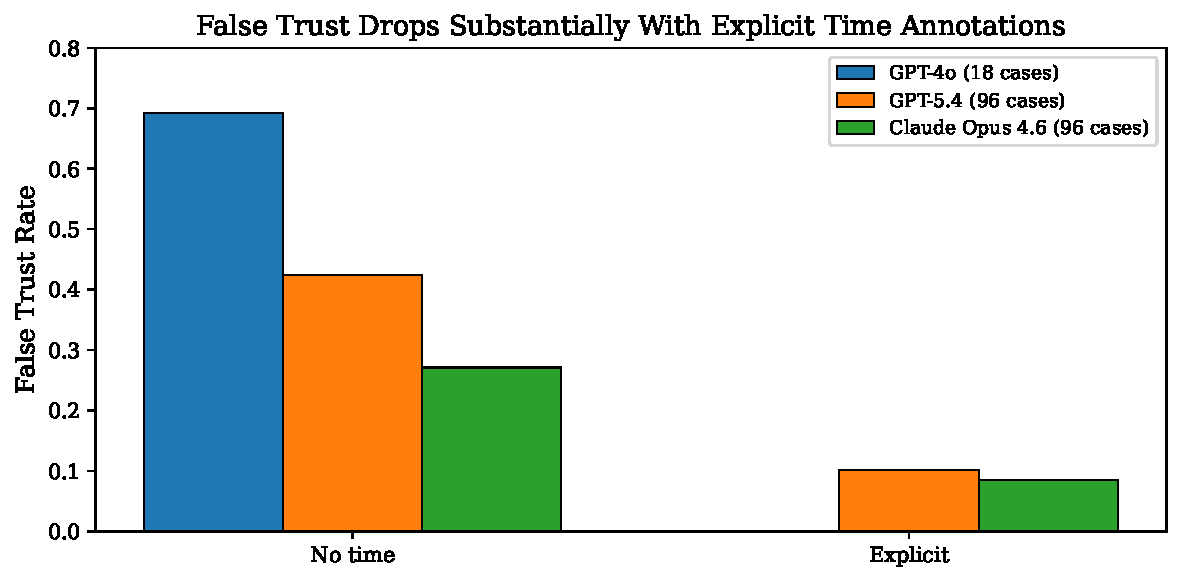
\includegraphics[width=0.85\textwidth]{fig2_false_trust.pdf}
\caption{False trust rate across prompting conditions for the three most capable models. Without time annotations, models trust stale information 69--100\% of the time. Explicit annotations reduce this to 0\%.}
\label{fig:false_trust}
\end{figure}

\subsection{Finding 2: Explicit Annotations Substantially Reduce the Blind Spot}

Adding a clearly labelled elapsed-time annotation (``Time since this information was observed: 4 hours ago'') produces large improvements:

\begin{itemize}
    \item \textbf{GPT-5.4} (96 cases): 5.1\% $\to$ 66.1\%. False trust: 42.4\% $\to$ 10.2\%.
    \item \textbf{Claude Opus 4.6} (96 cases): 0\% $\to$ 64.4\%. False trust: 27.1\% $\to$ 8.5\%.
    \item \textbf{Claude Sonnet 4} (96 cases): 0\% $\to$ 62.7\%. False trust: 39.0\% $\to$ 6.8\%.
    \item \textbf{GPT-4o} (96 cases): 3.4\% $\to$ 40.7\%. False trust: 33.9\% $\to$ 13.6\%.
\end{itemize}

The temporal reasoning capability exists latently in these models.
It requires only the right framing -- a clearly labelled elapsed-time annotation -- to activate.

\begin{figure}[t]
\centering
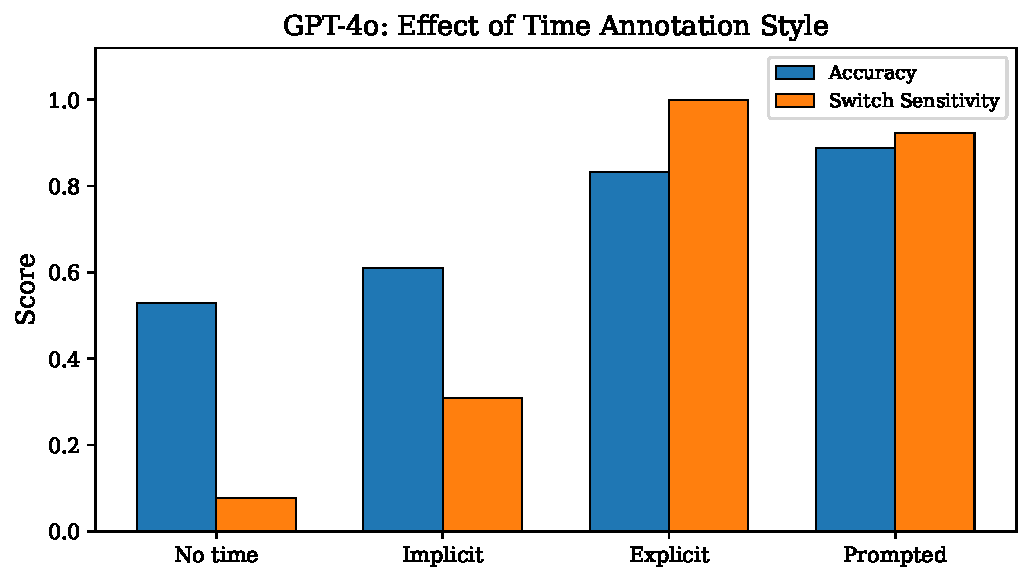
\includegraphics[width=0.75\textwidth]{fig4_gpt4o_conditions.pdf}
\caption{GPT-4o performance across four prompting conditions. Implicit time yields only partial improvement; explicit time produces the full effect.}
\label{fig:gpt4o_conditions}
\end{figure}

\subsection{Finding 3: Implicit Timestamps Are Insufficient}

Simply mentioning elapsed time casually (``observed 3 hours ago'' in a context header) yields only partial improvement.
GPT-4o reaches 30.8\% switch sensitivity with implicit time vs.\ 100\% with explicit.
Claude Sonnet reaches 15.4\% vs.\ 76.9\%.

The temporal signal must be \emph{salient} -- clearly labelled and separated from the content -- to be effective.
Burying a timestamp in metadata is not enough.

\subsection{Finding 4: Prompting About Staleness Does Not Help}

The prompted condition adds a system-level instruction: ``Before answering any question, consider whether the available information might be outdated.''
One might expect this metacognitive prompt to help.
In practice, it does not consistently improve on explicit time alone.

For GPT-5.4, prompting halves switch sensitivity compared to explicit time alone (46.2\% vs.\ 84.6\%).
For Claude Sonnet, unnecessary refresh rises from 14.3\% to 33.3\%.
For Claude Haiku, unnecessary refresh reaches 52.4\% -- it refreshes everything, including birthdays and capital cities.

The time annotation itself, not instructions about how to use it, appears to be the active ingredient.

\begin{figure}[t]
\centering
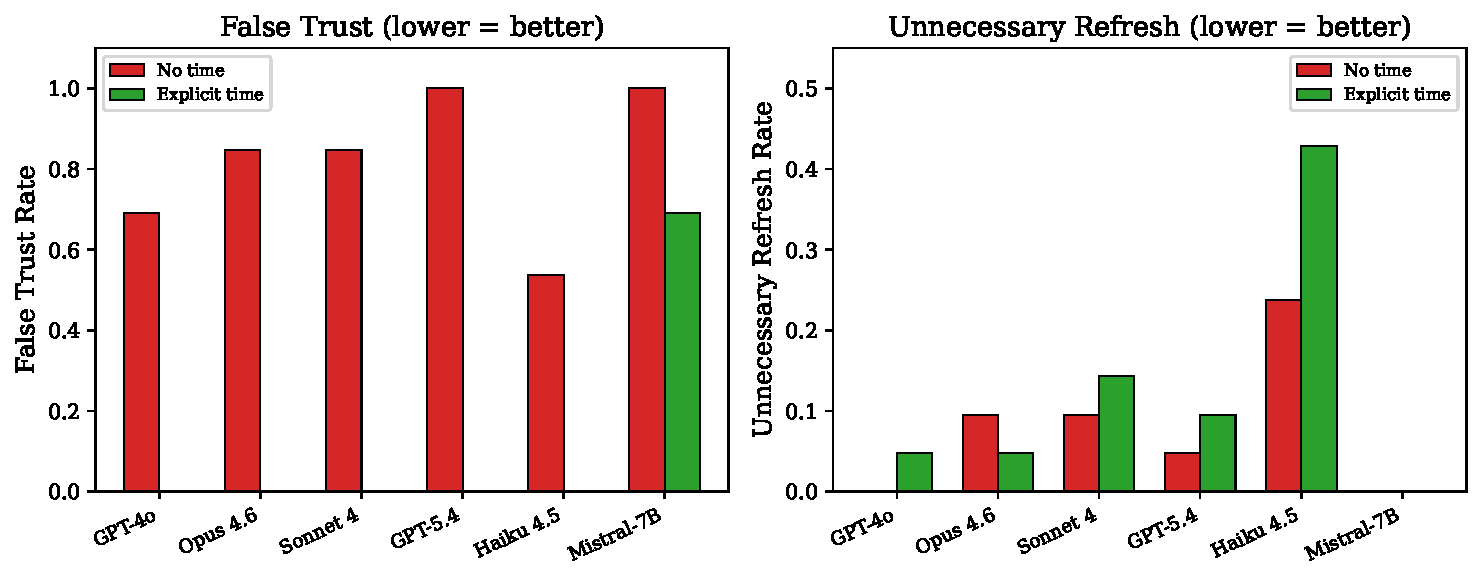
\includegraphics[width=\textwidth]{fig3_tradeoff.pdf}
\caption{The staleness-caution tradeoff. Time annotations eliminate false trust (left) but increase unnecessary refreshing of stable facts (right), especially for smaller models like Haiku and Mistral.}
\label{fig:tradeoff}
\end{figure}

\subsection{Finding 5: Smaller Models Over-Correct}

Claude Haiku and Mistral-7B reveal a \emph{staleness-caution tradeoff}.
Upon receiving time annotations, they begin refreshing indiscriminately -- stable facts and volatile facts alike.
Haiku's overall accuracy actually \emph{decreases} in the prompted condition (from 58.8\% to 52.8\%) despite eliminating false trust, because it trades dangerous trust for excessive caution.

Mistral-7B in the prompted condition is the extreme case: it refreshes 100\% of the time, achieving 0\% false trust but 100\% unnecessary refresh.
It has adopted a ``when in doubt, refresh'' policy rather than calibrating against fact volatility.

This suggests that the temporal blind spot has two components: (1) detecting that context has age at all (addressed by annotations), and (2) calibrating refresh thresholds against fact stability (which may require either more capable models or task-specific fine-tuning).

% ============================================================
\section{Cross-Model Analysis}
\label{sec:cross}

Table~\ref{tab:cross} summarises switch sensitivity across all seven models.

\begin{table}[h]
\centering
\caption{Switch sensitivity by model in the no-time condition vs.\ the explicit-time condition. Models with 96-case results are shown on the generated benchmark; others on the 18-case hand-crafted set. The blind spot is consistent across all models; the benefit of annotation varies.}
\label{tab:cross}
\begin{tabular}{lccc}
\toprule
\textbf{Model} & \textbf{Cases} & \textbf{No Time} & \textbf{Explicit Time} \\
\midrule
Mistral-7B (local) & 18 & 0.0\% & 30.8\% \\
GPT-4o-mini & 18 & 0.0\% & 53.8\% \\
Claude Haiku 4.5 & 18 & 0.0\% & 38.5\% \\
\midrule
GPT-4o & 96 & 3.4\% & 40.7\% \\
Claude Sonnet 4 & 96 & 0.0\% & 62.7\% \\
GPT-5.4 & 96 & 5.1\% & 66.1\% \\
Claude Opus 4.6 & 96 & 0.0\% & 64.4\% \\
\bottomrule
\end{tabular}
\end{table}

Two patterns stand out:

\paragraph{The blind spot does not diminish with scale.}
GPT-5.4, the most capable model tested, shows 7.7\% switch sensitivity without time -- no better than GPT-4o.
Within our evaluation, temporal sensitivity to cached context age does not appear to be an emergent capability.
It must be explicitly provided in the input.

\paragraph{The benefit of annotation scales with capability.}
While all models improve with explicit time annotations, the magnitude of improvement correlates with model capability: On the 96-case generated benchmark, GPT-5.4, Claude Opus 4.6, and Claude Sonnet reach 63--66\%, GPT-4o reaches 41\%, while Mistral-7B reaches 31\% on the hand-crafted set.
More capable models appear to have stronger latent temporal reasoning that activates more fully when given explicit elapsed time.
This is consistent with a \emph{representation bottleneck}: the reasoning ability is present, but requires the right input format to engage.

% ============================================================
\section{Discussion}
\label{sec:discussion}

\paragraph{Representation gap, not reasoning gap.}
The most striking aspect of our results is the size of the no-time to explicit gap.
On the 96-case generated benchmark, GPT-5.4 goes from 5.1\% to 66.1\% switch sensitivity, Claude Opus 4.6 from 0\% to 64.4\%, and Claude Sonnet from 0\% to 62.7\%.
These models clearly possess substantial ability to reason about temporal context -- they simply do not apply it unless elapsed time is surfaced explicitly.

We hypothesise that this is because training data contains abundant timestamps as \emph{facts about events} (``The meeting is at 3 PM'') but rarely presents elapsed time as a \emph{decision signal about context reliability} (``This information is 4 hours old and may be unreliable'').
Models learn to process temporal expressions syntactically, but do not learn to use elapsed time as a cue for context trustworthiness.

This interpretation is consistent with but not proven by our data.
Alternative explanations include prompt formatting effects (explicit annotations may simply draw attention to any metadata, temporal or otherwise) or position effects (the annotation appears in a salient location in the prompt).
Disentangling these would require further controlled experiments, such as adding non-temporal metadata in the same position to test whether the effect is specific to time.

\paragraph{Implications for deployed systems.}
Our results suggest that RAG systems, tool-using agents, and caching layers that serve previously observed information to language models could benefit from elapsed-time annotations.
Three concrete interventions follow:
\begin{enumerate}
    \item \textbf{RAG pipelines} could annotate retrieved passages with ``Retrieved: [time] ago.''
    \item \textbf{Tool-using agents} could tag tool outputs with ``Observed: [time] ago.''
    \item \textbf{Context caches} could include elapsed-time metadata in the prompt, not just in system logs.
\end{enumerate}
These are lightweight engineering changes at the prompt layer that require no model retraining.
The expected benefit, based on our results, is a substantial increase in temporal sensitivity for the most capable models.
Whether the effect generalises to production workloads and more naturalistic scenarios remains to be validated.

\paragraph{The staleness-caution tradeoff.}
Time annotations introduce a new failure mode: over-refreshing stable facts.
This is most pronounced in smaller models (Haiku, Mistral-7B) and in the prompted condition.
Practically, this means that adding elapsed-time annotations may increase API costs for tool-using agents that now refresh more aggressively.
In most settings, this tradeoff favours annotation: false trust in stale information is typically more harmful than an unnecessary refresh.
A user who receives stale information presented as current may make costly decisions; an agent that makes an extra API call merely incurs latency.

\paragraph{Limitations.}
Our evaluation has several limitations that should inform interpretation of the results.

\emph{Scale:} Five models are evaluated on 18 hand-crafted scenarios; four (GPT-4o, GPT-5.4, Claude Sonnet, Claude Opus 4.6) are additionally evaluated on a larger 96-case generated benchmark.
Effect sizes are smaller on the generated benchmark (41--66\% vs.\ 31--100\% on hand-crafted), suggesting the hand-crafted scenarios may overstate the effect for some models.
Evaluating the remaining models (Haiku, GPT-4o-mini, Mistral) on the larger benchmark is straightforward but not yet completed.

\emph{Ecological validity:} Our scenarios are realistic but synthetic.
We do not test in deployed RAG or agent systems, where models must jointly reason about content relevance, temporal freshness, and user intent.
The effect may be smaller or larger in naturalistic settings.

\emph{Prompt confounds:} Adding ``Time since observed: X'' changes more than just the temporal signal -- it also changes prompt length, structure, and the presence of a labelled metadata field.
We partially control for this with the implicit condition (which adds temporal information without a labelled field) and the prompted condition (which adds a system instruction without temporal data), but a fully controlled design would require non-temporal metadata baselines.

\emph{Coverage:} The evaluation is zero-shot and English-only. Few-shot examples might partially close the no-time gap by teaching models to attend to temporal cues. The blind spot may manifest differently in other languages.

\emph{Single turn:} We test single-turn temporal reasoning. Multi-turn scenarios where staleness accumulates or evolves over a conversation remain untested.

% ============================================================
\section{Conclusion}

Across the models and stale-context tasks we tested, language models show near-zero sensitivity to elapsed time (0--8\%) unless age is explicitly represented in the prompt.
Adding a single natural-language annotation of how long ago information was observed raises sensitivity to 31--66\% on a diverse generated benchmark (and higher on hand-crafted scenarios), with false trust dropping from 27--42\% to 7--14\% for the most capable models.

This pattern is consistent across seven models from three providers, spanning four capability tiers and two benchmark sizes (18 hand-crafted and 96 generated scenarios).
It does not diminish with scale: GPT-5.4 shows the same near-zero baseline sensitivity as smaller models.
The fix requires no model retraining, no architectural changes, and no special tokens -- only a change at the prompt layer.

We believe these results motivate a simple engineering recommendation: any system that presents previously observed information to a language model should annotate it with elapsed time.
Further work is needed to validate this recommendation in deployed agent and retrieval systems, with larger scenario sets and in naturalistic settings.

\paragraph{Reproducibility.}
All evaluation code, prompts, test scenarios, and raw model responses are available at \url{https://github.com/neilt93/temporal-bench}.

% ============================================================
\bibliographystyle{plainnat}
\bibliography{references}

\end{document}
